%!TEX root = ../../fourthYearReport.tex
\paragraph{Work package 2 progress}


% Morteza
\subparagraph*{CoM dynamic manipulability as a tool to study, analyze and measure physical abilities of humans and robots}
As part of T2.2 and also T2.3, UB continued on improving CoM dynamic manipulability as a tool to study, analyze and measure physical abilities of humans and robots.  First, the equation for the CoM manipulability ellipsoid was modified to decompose the effect of velocity and gravity related accelerations from the configuration dependent parts.  Then, two different
choices for the weighting matrix were introduced in order to evaluate the physical ability to accelerate the CoM with certain limits at the joint torques or joint accelerations.
\bigskip

\textbf{Progress}\\
Assuming unit weighted norm of actuated joint torques as
%
\begin{equation}
\Btau^T \BW_\tau \Btau = 1 \, ,
\label{tauWtau=1}
\end{equation}    
%
the modified inequality of the CoM manipulability ellipsoid is
%
\begin{equation}
0 \le (\ddot{\Bc} - \ddot{\Bc}_{vg})^T (\BJ_\tau \BW_\tau^{-1}
\BJ_\tau^T)^{-1} (\ddot{\Bc} - \ddot{\Bc}_{vg}) \le 1 \, ,
\label{torqueellipse}
\end{equation}
%
where $\BW_\tau$ is the weighting matrix and $\ddot{\Bc}$ is the CoM
acceleration as
%
\begin{equation}
\ddot{\Bc} = \BJ_\tau \Btau + \ddot{\Bc}_{vg} \, ,
\label{cdd}
\end{equation}
%
$\BJ_\tau$ is a Jacobian that maps joint torques to the CoM acceleration and
$\ddot{\Bc}_{vg}$ is the velocity and gravity dependent part of the CoM
acceleration.  The center of this ellipsoid is $\ddot{\Bc}_{vg}$ and its radii
and orientation can be determined by the eigenvectors and eigenvalues of
matrix $(\BJ_\tau \BW_\tau^{-1} \BJ_\tau^T)$.  Therefore, the size and shape
of ellipsoid is configuration dependent only.  Velocity and gravity only alter
the location of the ellipsoid within the space of the CoM acceleration.

Different choices can be used for $\BW_\tau$ based on the application.  Here,
we discuss two reasonable choices that can be used for general purposes.\\

\textbf{First Choice: Torque Limits}\\
\label{subsec:1stchoice}
Our first proposed reasonable choice for $\BW_\tau$ is
%
\begin{equation}
\BW_\tau^{-1} = \textrm{diag} ([k \Btau_{1_{max}}^2, k \Btau_{2_{max}}^2,
\ldots, k \Btau_{k_{max}}^2]) \, ,
\label{W_tau}
\end{equation}
%
where $\Btau_{i_{max}}$ is the saturation limit at the i$^{th}$ joint ($i = 1,
2, ..., k$) and $|\Btau_i| \leq \Btau_{i_{max}}$.  By using this weighting
matrix, (\ref{tauWtau=1}) will become
%
\begin{equation}
\frac{\Btau_1^2}{\Btau_{1_{max}}^2} + \frac{\Btau_2^2}{\Btau_{2_{max}}^2} +
\cdots + \frac{\Btau_k^2}{\Btau_{k_{max}}^2} = k \, .
\label{maxtorque_norm}
\end{equation}
%
Since the ellipsoid in (\ref{maxtorque_norm}) accommodates all combinations of
available joint torques (i.e.  $\Btau_i^2 / \Btau_{i_{max}}^2\leq 1$), the
outcome ellipsoid in (\ref{torqueellipse}) will include all achievable
accelerations of the CoM.
%
\begin{figure}
	\centering 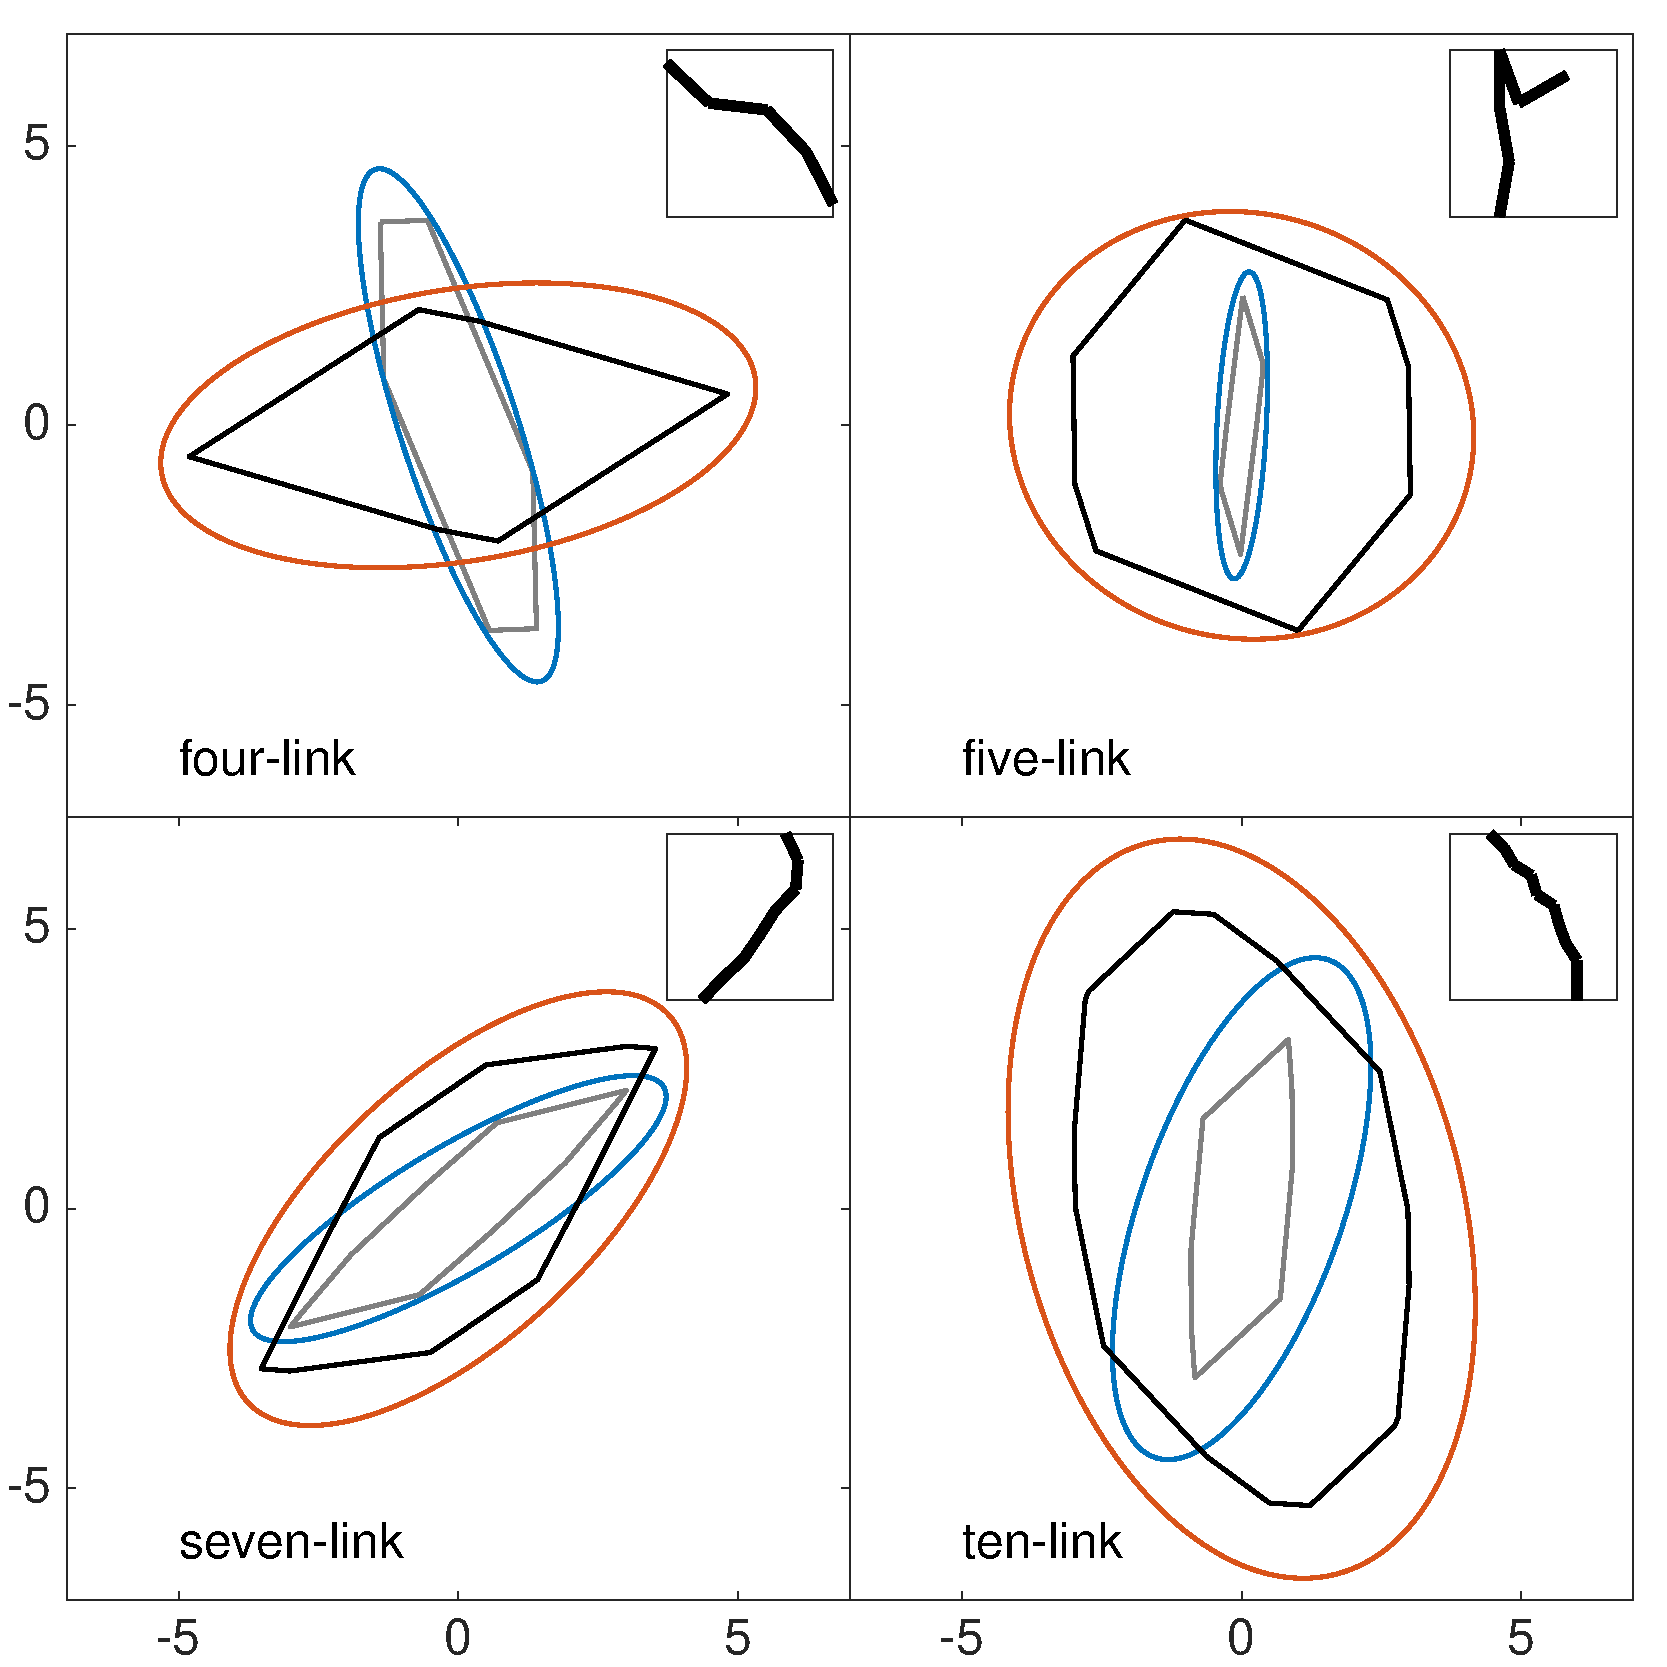
\includegraphics[width=.5\textwidth]{all.pdf}
	\caption{Feasible CoM acceleration polygons due to torque limits and CoM
		dynamic manipulability ellipses for four different planar robots.  The
		black polygons and red ellipses are for constrained end-effectors whereas
		the grey polygons and blue ellipses are for unconstrained robots at the
		same configuration.  The gravity and velocity are assumed to be zero
		($\ddot{\Bc}_{vg}=0$).}
	\label{torque_ellipses}
\end{figure}
%

In order to verify our choice of $\BW_\tau$ and to illustrate the relationship
between manipulability ellipsoid (ellipse in 2D) by using (\ref{W_tau}) and
achievable CoM accelerations due to torque limits, we plot ellipses for four
different planar robots at zero velocity and gravity
(i.e. $\ddot{\Bc}_{vg}=0$), assuming arbitrary torque limits.  These four
robots consist of (i) four, (ii) five, (iii) seven and (iv) ten links which
are connected to each other by active revolute joints.  The first link of each
robot is fixed to the ground by a passive revolute joint.  Each link is
assumed to have unit mass and length and its CoM in the middle.  Corresponding
robots configurations, which are chosen randomly, are depicted in the top
right corner of each plot.  Areas of feasible CoM accelerations (due to
saturation limits) for these robots are indicated in
Fig.~\ref{torque_ellipses} by grey and black polygons.  These polygons are
obtained numerically by mapping points inside the range of available joint
torques ($|\Btau_i| \leq \Btau_{i_{max}}$) to the CoM acceleration space.
This mapping is done by using (\ref{cdd}).  Both polygons for each robot are
for a same configuration.  The difference is that the black one shows the
achievable area when the end point of the last link is fixed (i.e. an extra
bilateral constraint).  This is to show the effect of an additional constraint
on feasible CoM accelerations (and also on ellipses).  The extra constraint
deforms the feasible area due to (i) the additional kinematic constraint
limiting the movements of the CoM in some directions, and (ii) contact forces
provide additional torques in some directions.  Corresponding manipulability
ellipses, which are calculated by using the weighting matrix in (\ref{W_tau}),
are also shown in Fig.~\ref{torque_ellipses}.  Red and blue ellipses are
related to constrained and unconstrained last links, respectively.  Comparing
the ellipses and polygons, it can be seen that, by employing (\ref{W_tau}) as
a weighting matrix, these ellipses can provide reasonable approximations of
achievable CoM accelerations.  It is obvious that calculating ellipses is
computationally much more efficient rather than obtaining polygons.  Ellipses
also provide analytical metrics which can be used to study and optimize a
robot's physical ability to manipulate its CoM.
%
\begin{figure}
	\centering
	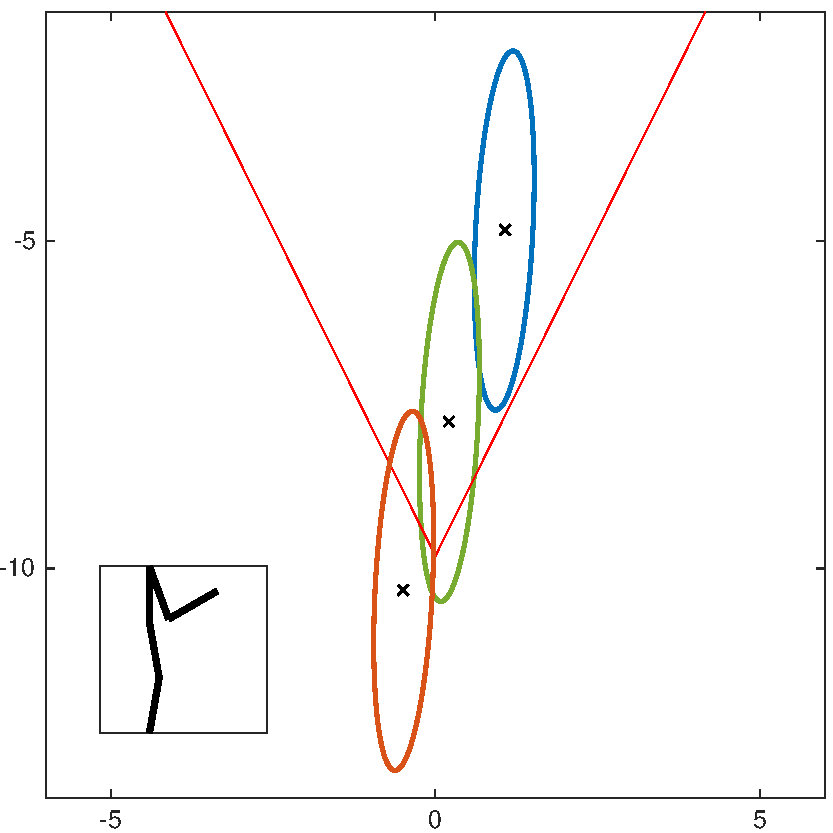
\includegraphics[width=.5\textwidth]{friction_cone.pdf}
	\caption{CoM dynamic manipulability ellipses for a five-link planar robot in
		different velocities.  The robot's configuration is shown on the bottom
		left corner.  Straight lines show the friction cone of the contact force.}
	\label{friction_cone}
\end{figure}
%

Including gravity and velocity to the above examples will only change center
points of the polygons and ellipses and will have no effect on shapes and
sizes of those areas.  As an example, we consider the five-link robot in the
same configuration and same torque limits as we had for the ellipses in the
top right corner of Fig.~\ref{torque_ellipses}.  The robot's configuration is
shown in the bottom left corner of Fig.~\ref{friction_cone}.  The blue ellipse
in this figure is the CoM manipulability ellipse for this robot when the
gravity exists and velocity is zero.  Therefore, the difference between this
ellipse and the blue one in the top right corner of Fig.~\ref{torque_ellipses}
is due to the gravity which only moves the center point ($\ddot{\Bc}_{vg} \neq
0$).  The red and green ellipses in Fig.~\ref{friction_cone} are also for the
same robot and same configuration but different velocities.  This implies a
kind of decoupling between the effects of inertial parameters and
configuration (size and shape of the ellipse) on one hand and velocity
(location of the ellipse) on the other hand.  This decoupling is important in
studying physical ability of a robot in different configurations independent
of its velocity.

The inequality (\ref{torqueellipse}) for the CoM dynamic manipulability
ellipsoid is derived assuming that the contacts are bilateral.  Although in
legged robots the contacts are usually unilateral, it is desired to maintain
the contacts (except contact switching) and prevent sliding or loss of contact
during the robot's performance.  Therefore, bilateral contact assumption still
makes sense if the contact forces satisfy the unilateral contact constraints.
In the example in Fig.~\ref{friction_cone}, replacing the bilateral constraint
by a unilateral one in the first link, we can draw friction cone constraints
in the CoM acceleration space.  Straight lines in Fig.~\ref{friction_cone}
show the CoM acceleration limits due to the friction cone when the coefficient
of friction is $0.5$.  As can be seen in this figure, different velocities
result in different feasible areas for a same manipulability ellipse due to
the unilateral constraint.  It implies that, although the CoM dynamic
manipulability ellipse, which is an approximation of the robot's physical
ability to accelerate its CoM, remains the same, enabling the robot to exploit
that ability is dependent on velocity, as well.  Note that, a proper velocity
has to be determined by a controller (or a motion planner) in order to exploit
available ability of a robot to reach a certain acceleration of the CoM and
satisfy the contact conditions.
%
\begin{figure}
	\centering
	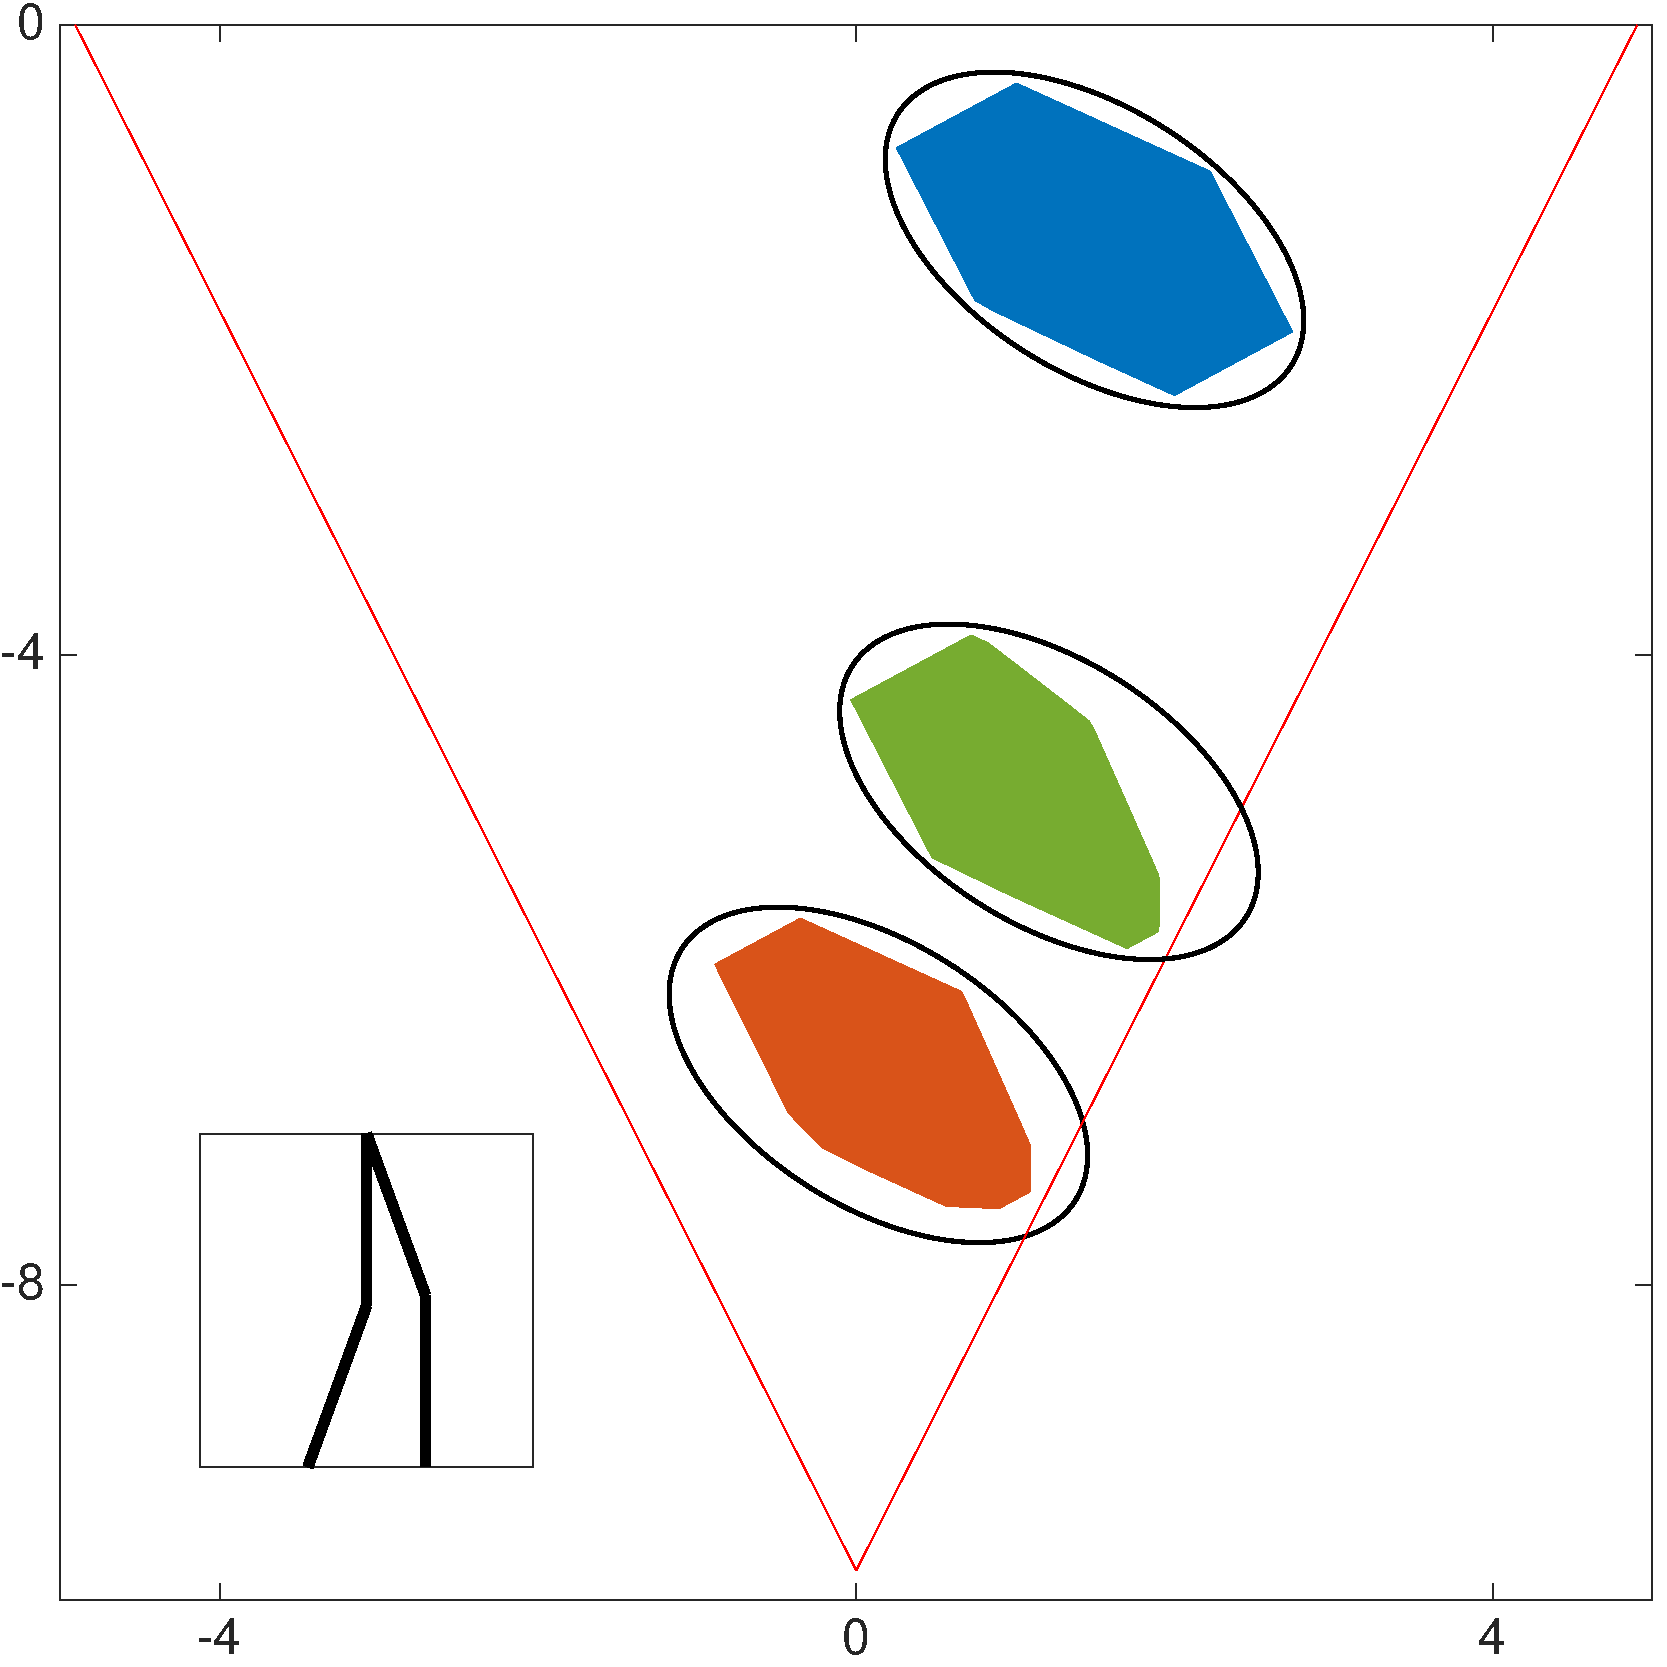
\includegraphics[width=.5\textwidth]{unilateral.pdf}
	\caption{CoM dynamic manipulability ellipses and feasible CoM acceleration
		polygons due to torque limits and unilateral constraints of a four-link
		robot with two contact points in different velocities.  Straight lines
		show the friction cone of the total force.}
	\label{unilateral}
\end{figure}
%

In the examples in Fig.~\ref{friction_cone}, we assumed a unilateral
constraint at the first link of the robot which is the same situation that
arises in single support phase for legged robots.  Since we also assumed that
the first joint is unactuated, the CoP (and also the ZMP) is always at the
contact point no matter if the robot is in balance or not.  This clarifies the
difference between the CoP (or the ZMP) and manipulability ellipses.  As can
be seen in Fig.~\ref{friction_cone}, ellipses provide information about the
robot's ability to accelerate the CoM in different directions with different
configurations and velocities, whereas the CoP (or the ZMP) remains at the
same point regardless of the robot's states.

It is worth mentioning that a larger ellipse means not only higher physical
ability to accelerate the CoM, but also larger feasible region for
$\ddot{\Bc}_{vg}$ to include a desired point in the CoM acceleration space
inside the ellipse.  In other words, although the ellipse's position and
therefore its feasible part due to the unilateral constraint is dependent on
$\ddot{\Bc}_{vg}$, having a larger ellipse provides more options for the
controller (or the planner) to choose a proper velocity to reach a desired CoM
acceleration.

Introducing more unilateral constraints to the robot (e.g. double support
phase in legged robots), or having multiple contacts which at least one of
them is unilateral, will result in velocity dependent limits for the CoM
acceleration.  In this case, each contact has its own friction cone limits
which are dependent on robot's states.  This is due to the relationship
between contact forces and robot's velocity.  Fig.~\ref{unilateral} shows
manipulability ellipses and their corresponding feasible CoM acceleration
areas of a four-link robot in three different velocities.  The polygons are
obtained numerically and by using (\ref{cdd}).  The robot's configuration is
depicted in the bottom left corner of the graph and it is chosen to mimic
double support phase of a planar biped.  The blue (top) area shows the
feasible area when the velocity is zero and the two others are for randomly
chosen velocities.  By comparing the three areas, it is obvious that different
limits are affecting feasible areas at different velocities which shows the
dependency of the limits on the robot's velocity.

As can be seen in Fig.~\ref{unilateral}, manipulability ellipses are the same
for all velocities implying that the robot's physical ability to accelerate
its CoM does not depend on velocity.  However, the robot's velocity affects
the feasibility of the areas due to the unilateral contacts.  In other words,
in all three velocities, the robot's physical ability to accelerate its CoM is
the same, although in two of the velocities (i.e. green and red areas) the
robot may lose its contact with the ground if it wants to reach certain
accelerations.  Therefore, exploiting robot's ability in a certain
configuration depends on choosing proper velocity by the controller (or
planner), as well.  Note that, straight lines in Fig.~\ref{unilateral} show
the friction cone limits for the total contact force which do not have any
effect on feasible areas at the chosen velocities since the areas are already
limited by friction cone constraints of individual contact forces.\\


\textbf{Second Choice: Joint Accelerations}\\
\label{subsec:2ndchoice}
Other than joint torques, joint accelerations are also important factors in
studying a robot's physical ability.  Obviously, producing less accelerations
at the joints, with same amount of joint torques and same CoM acceleration, is
desirable since it leads to lower joint velocities and consequently less joint
movements.  Less movements at the joints is beneficial since the robot's
workspace is limited.  Also lower joint velocities with same joint torques
means less work and higher energy efficiency.  Therefore, we introduce a
proper weighting matrix in order to study the robot's CoM acceleration due to
the limited joint accelerations.

Let $\BW_q \in \R^{n \times n}$ denote a symmetric positive definite matrix.
We define the second choice of $\BW_\tau$ as
%
\begin{equation}
\BW_\tau = \BJ_q^T \BW_q \BJ_q \, .
\label{W_tau,W_q}
\end{equation}
%
By substituting (\ref{W_tau,W_q}) into (\ref{tauWtau=1}), we will have
%
\begin{equation}
\Btau^T \BW_\tau \Btau = 1 = \Btau^T \BJ_q^T \BW_q \, \BJ_q \Btau \, .
\end{equation}
%
Given that $\ddot{\Bq} = \BJ_q \Btau + \ddot{\Bq}_{vg}$, the above equation
becomes
%
\begin{equation}
(\ddot{\Bq}-\ddot{\Bq}_{vg})^T \BW_q \, (\ddot{\Bq}-\ddot{\Bq}_{vg}) = 1 \,
,
\label{qddTWqdd=1}
\end{equation}
%
where $\BW_q$ can be used to unify the units or express the relative
importance of the joint accelerations in $\ddot{\Bq}$.  $\BJ_q$ is a Jacobian
that maps joint torques to the joint acceleration and $\ddot{\Bq}_{vg}$ is a
part of the joint accelerations due to gravity and joint velocities.  The
above equation specifies a n-dimensional ellipsoid in the joint acceleration
space which its center point is at $\ddot{\Bq}_{vg}$.  This point is the same
center point of a n-dimensional ellipsoid that will be obtained if we project
the unit weighted norm of joint torques (i.e. Eq.~(\ref{tauWtau=1})) to the
joint acceleration space.  Such ellipsoid will be the same as
(\ref{torqueellipse}) if we replace $\BJ_\tau$ with $\BJ_q$ and $\ddot{\Bc}$
with $\ddot{\Bq}$.

By choosing $\BW_\tau$ as in (\ref{W_tau,W_q}), CoM dynamic manipulability
ellipsoid will show an area in the CoM acceleration space which is achievable
via unit weighted norm of joint accelerations in (\ref{qddTWqdd=1}).
Therefore, by setting proper values for $\BW_q$ (user's choice based on the
application), a user can study the effect of joint accelerations on reaching
desired CoM accelerations.  As an illustrative example,
Fig.~\ref{two_ellipses} shows CoM manipulability ellipses for a five-link
planar robot (i.e. the same robot explained earlier in this section) in two
different configurations which are shown in bottom left corners of the plots.
Without losing generality, we set the gravity and velocity to zero in these
examples (i.e. $\ddot{\Bq}_{vg} = \ddot{\Bc}_{vg} = 0$).  Torque limits for
all four actuated joints are assumed to be one.  Green areas show feasible CoM
accelerations due to the torque limits and green ellipses are their
approximations which are obtained by using (\ref{W_tau}).  Blue and red areas
indicate CoM accelerations which are achievable by limited norm of the joint
accelerations.  For the blue areas the norm is one (i.e. $\ddot{\Bq}^T
\ddot{\Bq} = 1$) and for the red ones the norm is $3$ (i.e. $\ddot{\Bq}^T
\ddot{\Bq} = 9$).  Blue and red ellipses are obtained by using
(\ref{W_tau,W_q}) and setting $\BW_q$ to identity and $1/9$ times identity
matrices, respectively, to match the corresponding areas.  Green, blue and red
areas are obtained numerically and by using (\ref{cdd}).  In obtaining red and
blue areas corresponding joint acceleration limits (i.e. $\ddot{\Bq}^T
\ddot{\Bq} \leq 1$ for red areas and $\ddot{\Bq}^T \ddot{\Bq} \leq 9$ for blue
areas) are also considered.
%
\begin{figure}
	\centering
	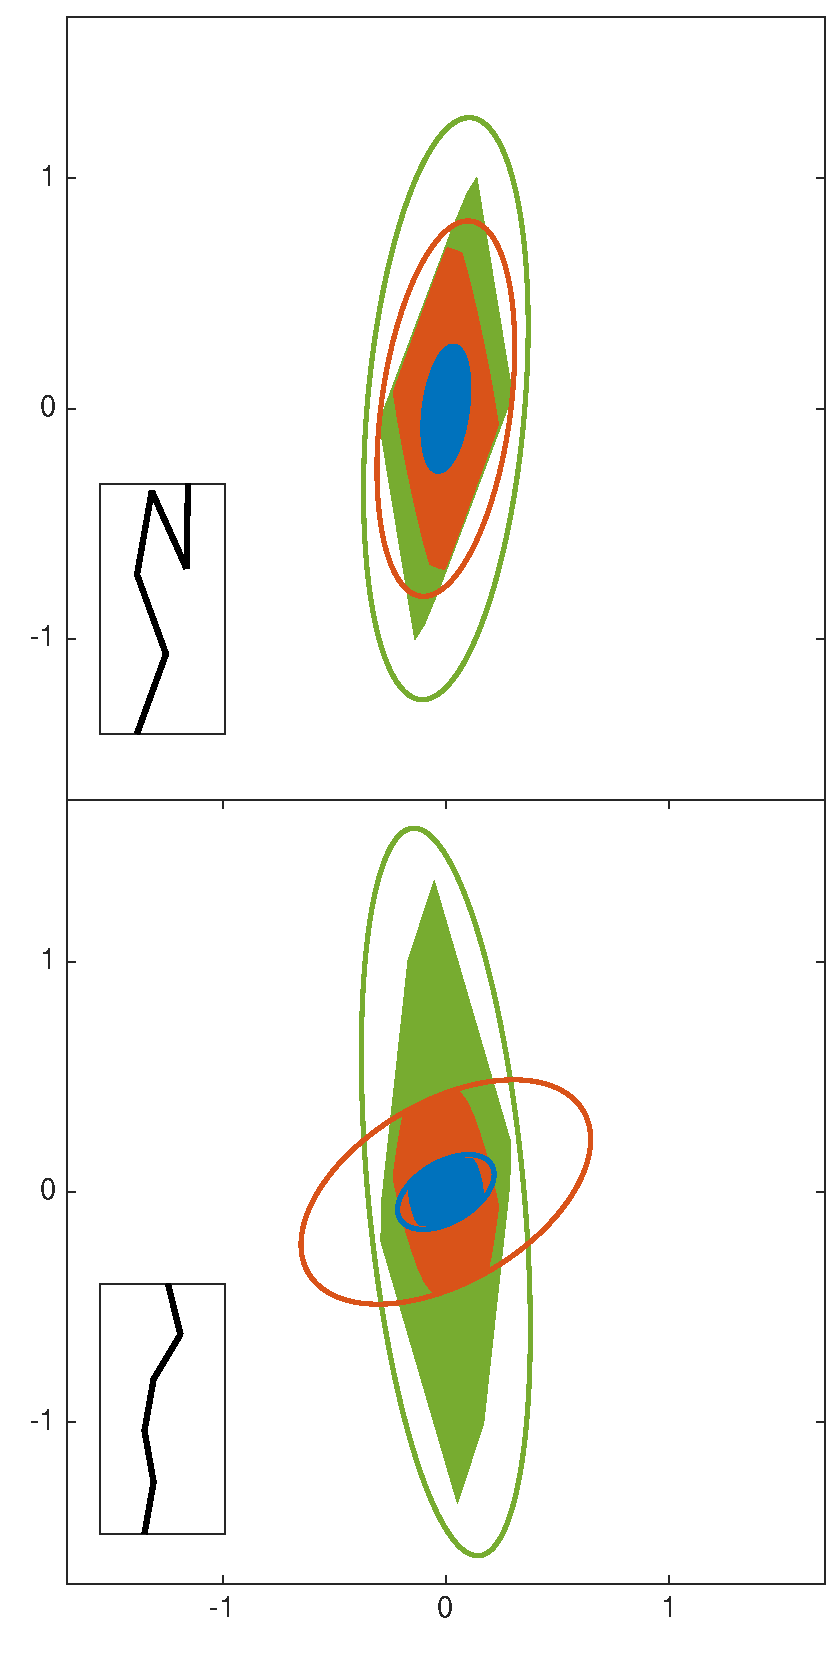
\includegraphics[width=.3\textwidth]{twoellipses.pdf}
	\caption{CoM dynamic manipulability ellipses with different weighting
		matrices for a planar five-link robot in two configurations.  Green areas
		show feasible CoM accelerations due to torque limits.  Blue and red areas
		show achievable CoM accelerations with unit weighted norms of joint
		accelerations.}
	\label{two_ellipses}
\end{figure}
%

As it is expected, and also can be seen in Fig.~\ref{two_ellipses}, blue and
red ellipses include all points in the blue and red areas, respectively.
Although they also include points which are not inside their corresponding
areas.  The reason is that the mapping from the joint acceleration space to
the CoM acceleration space is not one-to-one, which means that the mapping
from the CoM to the joint acceleration space may be different.  Comparing the
two examples in Fig.~\ref{two_ellipses}, it is obvious that in the top
configuration, although the green area is smaller, the blue and red areas are
larger compared to the bottom plot.  It means that, the same CoM accelerations
can be achieved by generating smaller accelerations at the joints in the top
configuration comparing with the bottom one.  This can be explained by CoM
dynamic manipulability ellipses as the blue and red ellipses are much more
aligned with the green one in the top plot rather than in the bottom one.
Note that, blue and red ellipses have the exact same alignments and the only
difference is in their sizes.  Therefore, in order to minimize the norm of the
joint accelerations to reach a certain CoM acceleration, one can minimize the
difference in the alignments of these two ellipses.

Since the proposed metric studies the motion of the CoM, which is the main
focus in balancing motions of robots, it can be used to evaluate a robot's
ability to balance.  Thus, we define \textit{physical ability to balance} as a
robot's physical ability to manipulate its CoM in the horizontal directions.
Therefore, if we project dynamic manipulability ellipsoids of a robot, in
different configurations, onto the horizontal plane, the configuration with
the largest ellipse (i.e. projected ellipsoid) will have the highest ability
to balance in the sense of the required torque if we use (\ref{W_tau}) or the
required joint accelerations if we use (\ref{W_tau,W_q}) .  Note that, the
largest projected ellipse is not necessarily the projection from the largest
ellipsoid, since the largest ellipsoid might be extended in another (i.e. the
vertical) direction.  Therefore, by using the CoM dynamic manipulability one
can compare different configurations of a robot] or even different robots in
terms of their physical abilities to maintain balance.


% chie
\subparagraph*{Human learning compliant force dynamics through physical interactions}
To explore the mechanism of human force perception has a key role in the CoDyCo project, aiming to provide natural and stable control for a humanoid robot in the similar manner with humans. Through this work,,an experimental design has been developed, and a series of human subject experiments examined the anticipated goal-directed behaviour interacting with different compliant force dynamics. Three different types of forces (a simple linear and two non-linear forces) were generated by a haptic device, and the human movements were measured against the compliant forces.The participants were asked to set the “half-position”  and“half-force”  after the certain repetitive movements to reach the target. The results showed that although humans were more sensitive to the position control than the force, they could differentiate the three dynamics. Interestingly humans seem to be more sensitive to the total power to the target than the point-force at the target.Moreover, the learning performance was also analysed and the learning curves were different between the three, suggesting some relations might exist in everyday real activities. As such, the work has deepened the understanding how humans perceive the force to reach anticipated goals ruled by the certain dynamics. This would be beneficial to apply it for providing not only natural human-robot interaction but also stable humanoid robot control when interacting with multiple compliant surfaces.

The study about human force perception and learning through compliant contact dynamics helps to design and develop a more natural and dynamical contact to humanoid robots. To explore the human learning compliant force dynamics through physical interactions, we generated four different compliant forces (two linear and two non-linear cases) by changing the stiffness values (See Figure \ref{fig:forcedyn}).

\begin{figure}[h!]
	\centering
	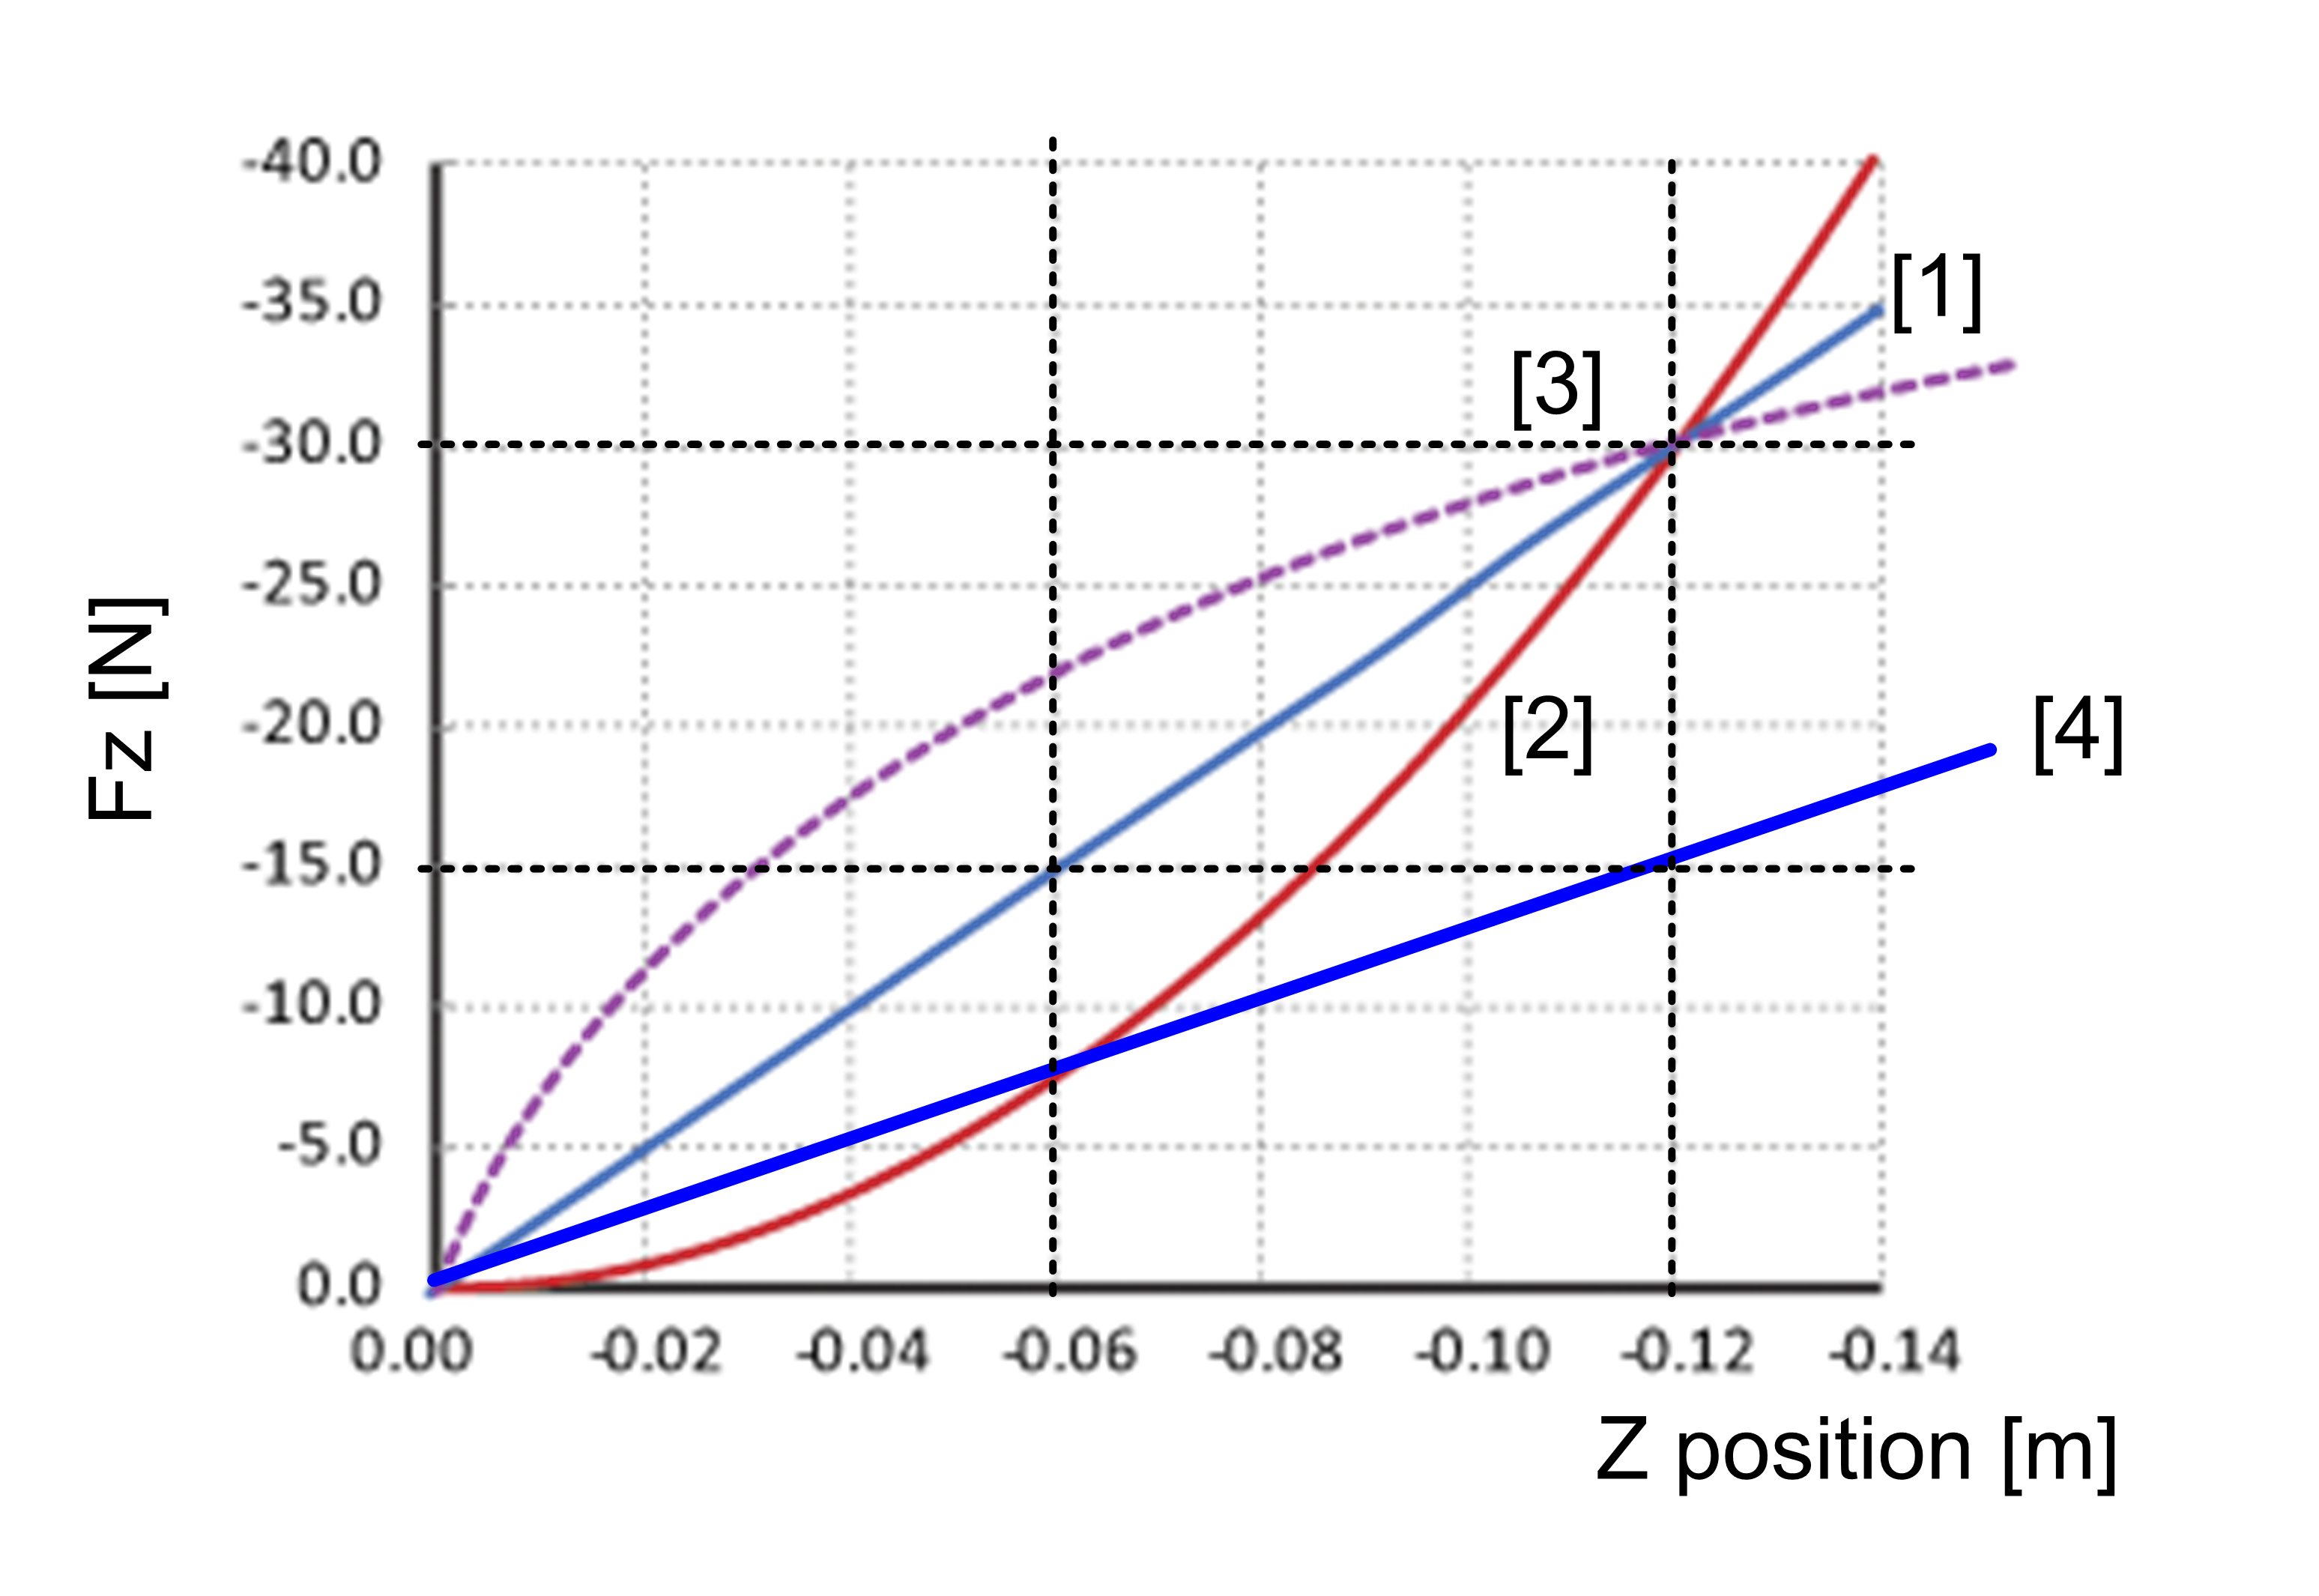
\includegraphics[width=.7\textwidth]{UB-Figure1.png}
	\caption{Four different force dynamics are applied. [1] Linear, [2] Non-linear (quadratic), [3] Non-linear (concave), and [4] Half-linear. The [1],[2],[3] are the same force at the end position (e.g., z=-0.12), and [2] and [4] are the same force at the half position  (e.g., z=-0.06).}
	\label{fig:forcedyn}
\end{figure}

\newpage

The stiffness values were calibrated depending on the goal position and the maximum force to be applied at this set position. The participants were asked to set the half-position and half-force after a certain repetition in order to be probed their responses whether or not they properly perceived the force dynamics. Figure \ref{fig:testrial} shows that although the performance tended to overshoot at both test trial due to the deprivation of the visual information of the target, the participants set the half-position in the similar manner regardless of the force dynamics. Conversely, there were significant differences between the three conditions at the half-force test trials.

\begin{figure}[h!]
	\centering
	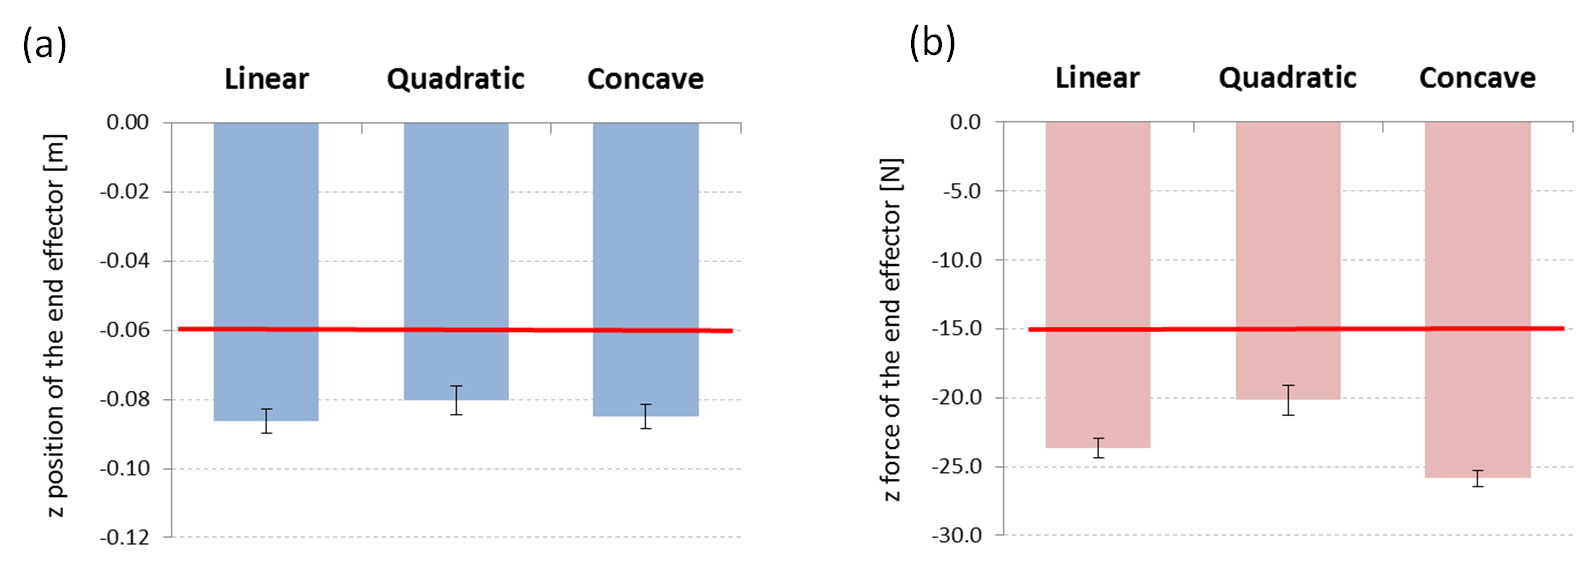
\includegraphics[width=.9\textwidth]{UB-Figure2.png}
	\caption{The test trial performances averaged across 18 participants.(a) the end-effector position at the test “half-position” trial and (b) the applied force at the test “half-force” trial. The red lines indicate the ideal values based on the dynamics (see Figure 1).}
	\label{fig:testrial}
\end{figure}

\bigbreak
\bigbreak
The dynamic learning evaluation revealed that there were significant differences between three forces in the learning performance averaged across 18 participants (see Figure \ref{fig:learnerror}). The concave force was not natural, and it was needed several repetitions to understand the dynamics and also to learn how to maintain the accuracy in reaching a target. In contrast, the linear force had less efforts but the learning model maintained a stable conditions after the repetitions. The quadratic force seemed to be a “well known or natural” force among the three,but still the performance gradually improved over the course of trials. These results suggest that the force model helps the user to achieve more precise and accurate movements.

\begin{figure}[h!]
	\centering
	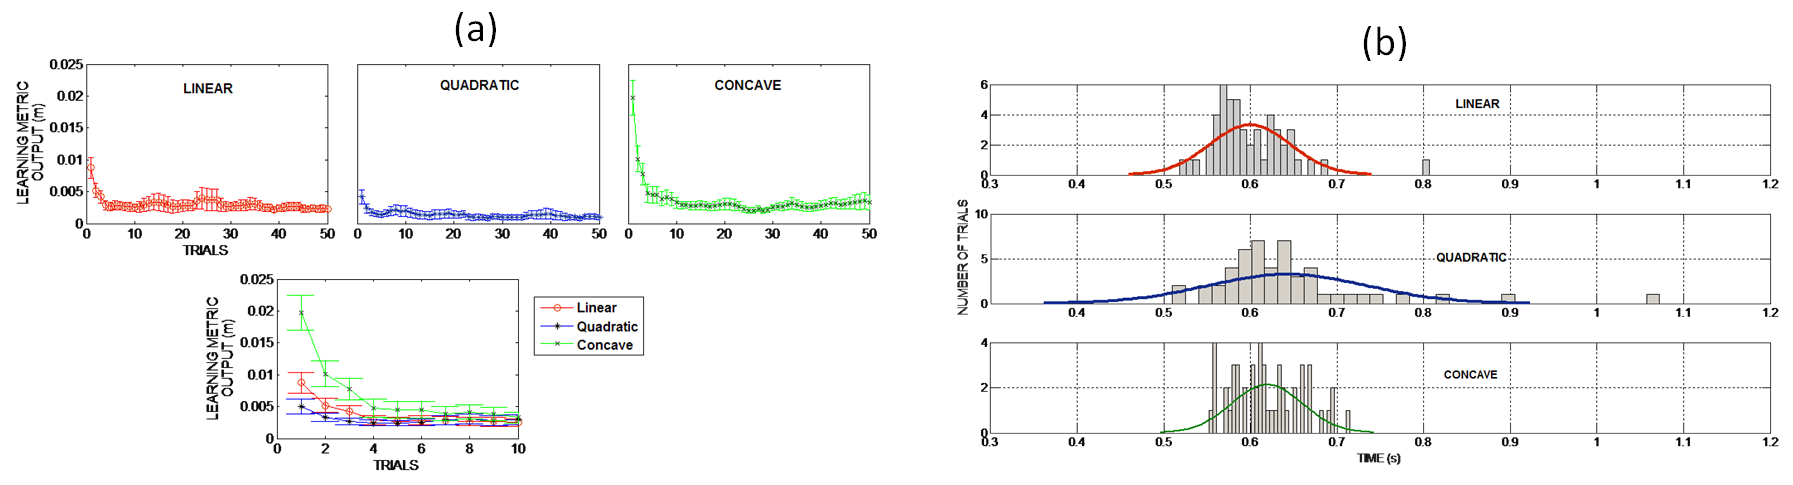
\includegraphics[width=.9\textwidth]{UB-Figure3.png}
	\caption{(a) Learning performance of the 18 participants along with the standard error. A big variation in the learning performance of the three different forces is observed within the initial 10 trials. 
		(b) Average time taken by the 18 participants to reach the target with the three different forces.}
	\label{fig:learnerror}
\end{figure}

% roberta
\subparagraph*{Tactile attention and memory in multi-finger contact}
Given CoDyCo’s focus on compliant contact with support surfaces under uncertainty, an important issue is the extraction of information about the contact surfaces through the sense of touch. Knowledge about surface texture, for example, roughness which affects friction and hence contact dynamics, may be derived from static or sliding contact. Two psychology studies at UOB have examined tactile roughness through perceptual judgments and brain activation, while a third study has examined the effects of tangential load force uncertainty on precision grip cooperative lifting.

People often use several digits simultaneously to touch surfaces. Thus, they may use two fingers (eg index and middle) side by side (e.g. in steadying themselves against a stable surface) or they might use thumb opposing the index (and possibly other fingers) to form a precision grasp on either side of an object (e.g. stair rail). Often the surfaces contacted by the two digits will be the same and the double contact affords improved tactile sensitivity over single contact. However, two surfaces that are not co-located may differ in texture. For example, when using precision grip to feel fabric, the “front” and “back” surfaces may have very different textures. The perceived texture of either surface is then likely to be affected by the surface on the reverse side. We have been investigating such contact in terms of interactive effects on roughness judgments arising from simultaneous contact with two separate surfaces. Depending on the two digits involved, we have shown attention and neural cross talk afford explanations of some of the effects seen \cite{roberts2010, roberts2013}. Within CoDyCo we have been contrasting two forms of perceptual judgment, based on single (magnitude estimation) and two successive presentations (2-interval forced choice) of the surfaces. The theoretical interest is in the potential role of short term tactile memory in the second case. Similarity of the two digit judgments despite differences in working memory requirements in the different perceptual tasks inclines us against a significant role for a memory component in multi-digit roughness perception. A paper is in preparation on this topic. 

\begin{figure}
	\centering
	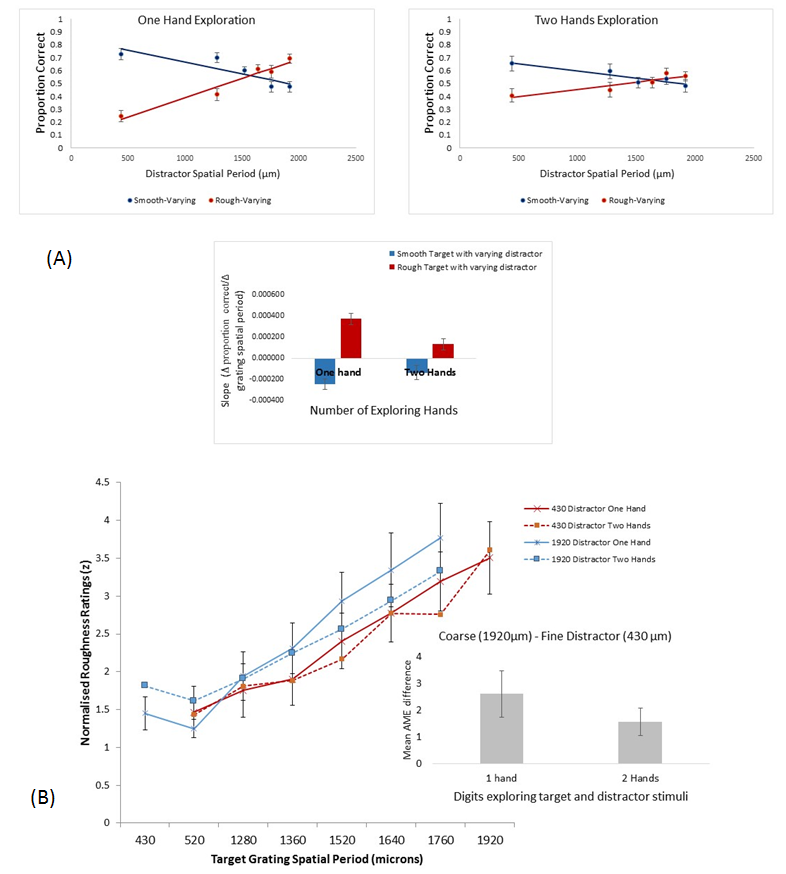
\includegraphics[width=.7\textwidth]{UB-r-Figure1.png}
	\caption{Multifinger contact effects on (A, above) 2-interval force choice (2-IFC) and (B, below) absolute magnitude estimates (AME) measures of roughness perception. In both tasks participants actively explored a target and distractor surface simultaneously using 2 digits; the digits were either on one hand or two hands, expected to result in more or less crosstalk. In the 2-IFC task (A), participants identified the rougher of a pair of target stimuli and were instructed to ignore the distracter. The red circles and line indicate group (N=12) average performance when the fine surfaced target was paired with various coarse distractor surfaces; a fine distractor depresses accuracy more than a coarse distractor. The blue circles and line show behaviour with the coarse target; a coarse distractor depresses accuracy more than does a fine one. The bar graph summarising mean slope across participants shows the distraction effect is greater in the one hand condition. 
		In the AME task (B), participants rated the roughness of target surfaces while instructed to ignore the simultaneously touched distractor. The graph at the top of figure 1b shows mean ratings for each target surface. The blue crosses and squares show mean ratings for each target surface with a coarse distractor surface. Mean ratings with a fine distractor surface are shown in red. It can be seen that a coarse distracter results in higher roughness ratings than does a fine distracter. As with 2-IFC, the distracter effects are greater with the distracter on the same hand as the target.}
	\label{fig:Multifingercontacts}
\end{figure}

\textbf{Surface roughness effects on brain activation in static and sliding contact}
Duplex theory proposes that surface roughness judgments are mediated by a combination of vibratory and spatial inputs from the slowly and rapidly adapting tactile mechanoreceptors \cite{Hollins2000}. Tactile processing by the brain primarily involves the somatosensory cortex. However, cortical areas primarily associated with auditory and visual input can also be involved. Thus, recently it has been shown that direct current stimulation of the visual or auditory cortex can facilitate spatial or temporal tactile judgments \cite{yau2014}. We are currently completing a brain imaging study in which we expect to demonstrate a neural basis for duplex theory. Thus we expect moving sliding textures will activate auditory cortex while static coarse textures invoke visual cortex; preliminary data in Figure 2 show auditory cortex activation with sliding contact.

\begin{figure}
	\centering
	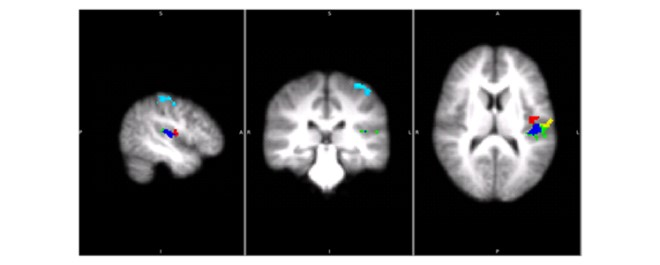
\includegraphics[width=.7\textwidth]{UB-r-Figure2.jpg}
	\caption{Activations during passive touch.  The three panels indicate sagittal, coronal and horizontal planar sections of the brain with multisensory activations for a tactile discrimination task contrasting coarse and fine texture perception under moving and static touch conditions. Regions of interest shown with coloured blobs, were more activated for moving (vs static) touch, including auditory cortex (TE1.0). The stimuli were applied to the right index finger of passive participants, N=13; Light blue: BA1, Green: OP1, Red: OP3, Yellow: OP4, Blue: TE1.0}
	\label{fig:ActivationsDuringPassiveTouch}
\end{figure}

\textbf{The role of uncertainty in shared control of grip in cooperative lifting}
Social processes in cooperative multi-person action is a major topic in psychology, but there has been very little analysis of kinematics and dynamics of joint action. We have been examining control of precision grip force during a 2-person lifting task in which the load to be lifted varies from trial to trial. There are three conditions that manipulate load uncertainty. In the first condition the weight is unknown to either participant. In the second condition it is known to just one of the participants, while in the third condition it is known to both of them.  We find systematic changes in anticipatory grip as a function of both one’s own knowledge but also what is known by one’s partner (see Figure \ref{fig:JointLiftingAction}).

\begin{figure}
	\centering
	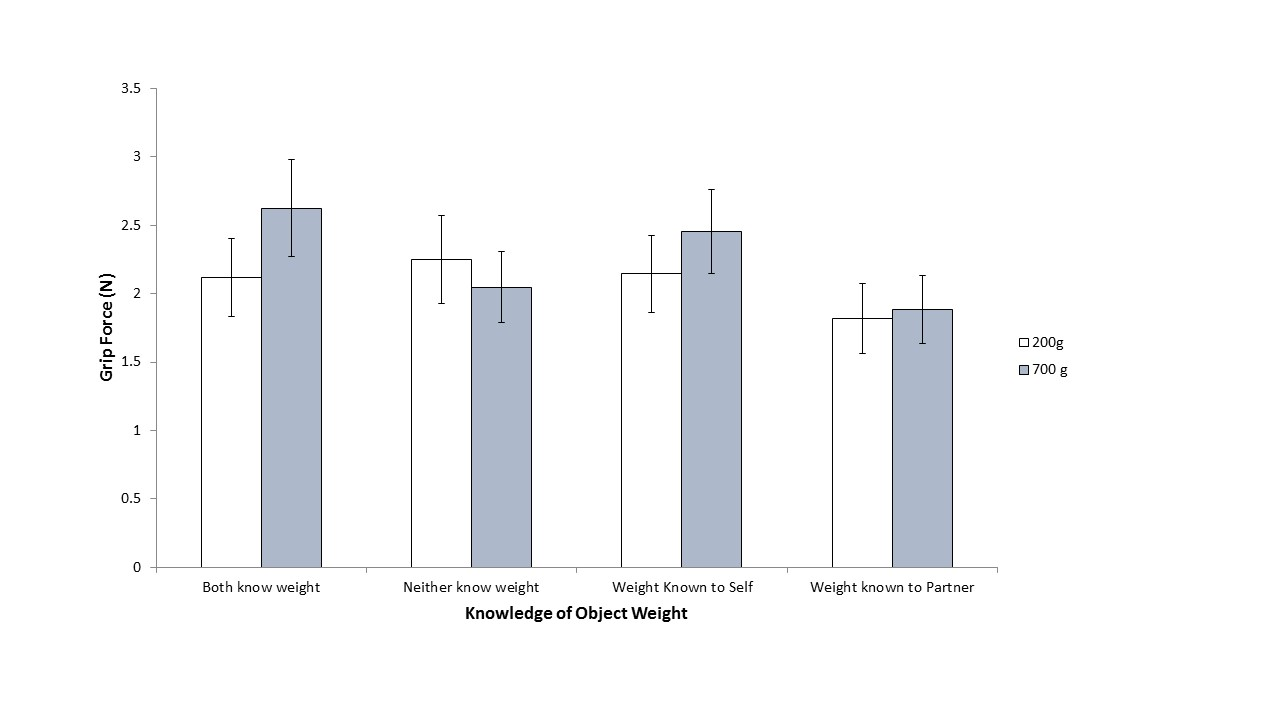
\includegraphics[width=.8\textwidth]{UB-r-Figure3.jpg}
	\caption{Joint lifting action. The participants worked in pairs to lift a bar to a target height. The weight at the centre of the bar (either 200g or 700g) was known to one, both or neither participant in pair. The force with which the participants held the bar in anticipation of a lift in the different knowledge conditions is shown along with on SE of the mean.}
	\label{fig:JointLiftingAction}
\end{figure}


% vijay
\subparagraph*{Human arm impedance characteristics in a dynamical contact task}
Studies on human behaviour models with specific relation the arm movement while performaing dynamical tasks have been used to understand the prinicples behind human arm impedance\cite{Darainy, Mussa-Ivaldi}. The effect of such impedance can be a result of the active forces (resisting or assisting) applied by the muscular reflexes, contractions and any specific joint limitations of the movement. From the literature, it is understood that the directional influence of such movements has a direct influence in the arm stiffnes or impedance specifically being anisotropic under static conditions \cite{Burdet2001}. These arm impedance characteristics have also been studied using a virtual model, while the human arm is trying to influence the virtual system by performing a dynamic task \cite{Tsuji2004}. Tee et al.,\cite{tee2004} developed a computational model to study the effect of human arm impedance and the joint stiffness measures observed while trying to perform a task in any given dynamic enviroment (stable or unstable). These studies focus mainly on the human arm impedance models in a static or dynamic task which will help understanding the human impedance perfromance in any enviroment. \\

As part of the CoDyCo project, the human behaviour model while in contact with compliant forces were analysed and studied previously. Further to this analysis, it is interesting to understand the similar behaviour while in contact with a robot model or any defined object with significant dynamic influence. These intentions led to the development of the following preliminary study which is perfromed using the Haptic master along with a simulated enviroment. The goal of this task is to understand how humans emulate or modify their course of action and perception in maintaining the postural balance of a robot model.  \\

\textbf{Methods}\\
The human arm impedance behaviour can be studied by constraining or limiting the human movement within a specific range. Further, a dynamic task is also needed which will encourage the human to engage in continuous movement. This continuous exploration and the variation in the human arm behaviour will help in understanding the principles behind the mechanical stiffness of the human arm. Further, to answer the global objective of the CoDyCo project, we designed the dynamical task as to help or assist the humanoid robot from a sitting position to the standing position. 

The robot model is designed as simple planar double inverted pendulum model which will vary its performance with respect to the velocity and the force parameters received from the Haptic master. The dynamic equation for an inverted pendulum model can be represented as  
\begin {equation}
\ddot{x}= g/m+F_{ext}/m+F_{con}/m
\end{equation}
$ F_{ext}$ is the external force received from the Haptic Master input and $F_{con}$ is the controller force (PD controller) in the knee joint (to maintain the constrained movement). The force applied by the human via the Haptic Master device, is transformed directly to the end-effector position of the planar robot model. The force applied at the end effector is then transformed to the individual joint torques using the following computation:
\begin{equation}
\tau=J^{T}*F_{ext}
\end{equation}
with $\tau$ being the joint torque to be applied in the hip, knee and ankle joints of the robot model. $F_{ext}$ corresponds to the force applied by the human and measured through the Haptic master device.\\
To maintain the initial sitting position of the joints the model needs to be equipped with a PID controller or a COM based balancing controller which will further act depending on the force applied by the human through the Haptic Master.  
\begin{figure}[h!]
\centering
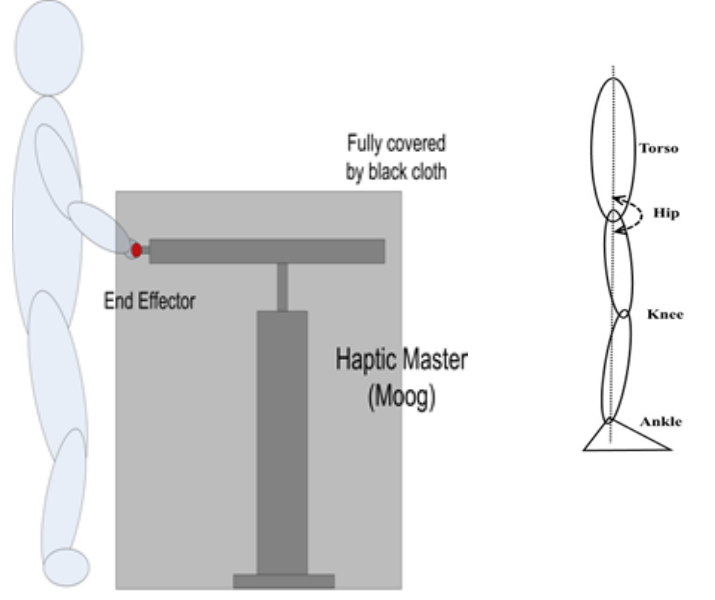
\includegraphics[width=.5\textwidth]{S2S.png}
\caption{ The spring model in the Haptic API is used to emulate the performance of a robot model (mass) and the human applies the force along the x and z directions similar to a planar movement which is visualized using the model in real time.}
\label{Humanarmimpedance}
\end{figure}


\textbf{Experimentation}\\
The experimental setup involves the Haptic Master device which helps in emulating the human applying the necessary force to initiate the robot (model) to move from a sitting position to standing position. A planar robot model is developed using Simulink and it is directly integrated with the x and z direction forces applied by the participants. The haptic master is also limited to the planar movement which helps the human in controlling the applied moment or contact force. A real time visualization of the planar model is displayed in the monitor which helps the participant to understand and to control the arm movements.  

Figure {\ref{Humanarmimpedance}} presents the experimental set-up used in this analysis, the Haptic Master moog and Simulation model. Participants will visualize the pendulum model as a visual feedback and can relate the change in the movement depending on the force applied. The static (iso-metric) force model is with high stiffness emulating the body weight and the force feedback from the human is taken as a direct input. 

\textbf{Preliminary Results}\\
A preliminary study was conducted to evaluate the objective of combining the dynamical task along with restricted human arm movement. This analysis help to understand the behaviour of the low level controller used in the model and influence of the human applied forces. Figure {\ref{externalforce}} illustrates the external force observed as a result of the applied forces along the x and z axis. The participant was performing a planar motion by applying force along the x and z axis within a given free space. The forces observed to be varying continuously which signifies the dynamically exploration of the user whilst maintining a higher forces. The real time visualization of the model helped the user to increase or decrease the forces along x and z directions such as to control the movement of the planar robot model.
\begin{figure}[h!]
\centering
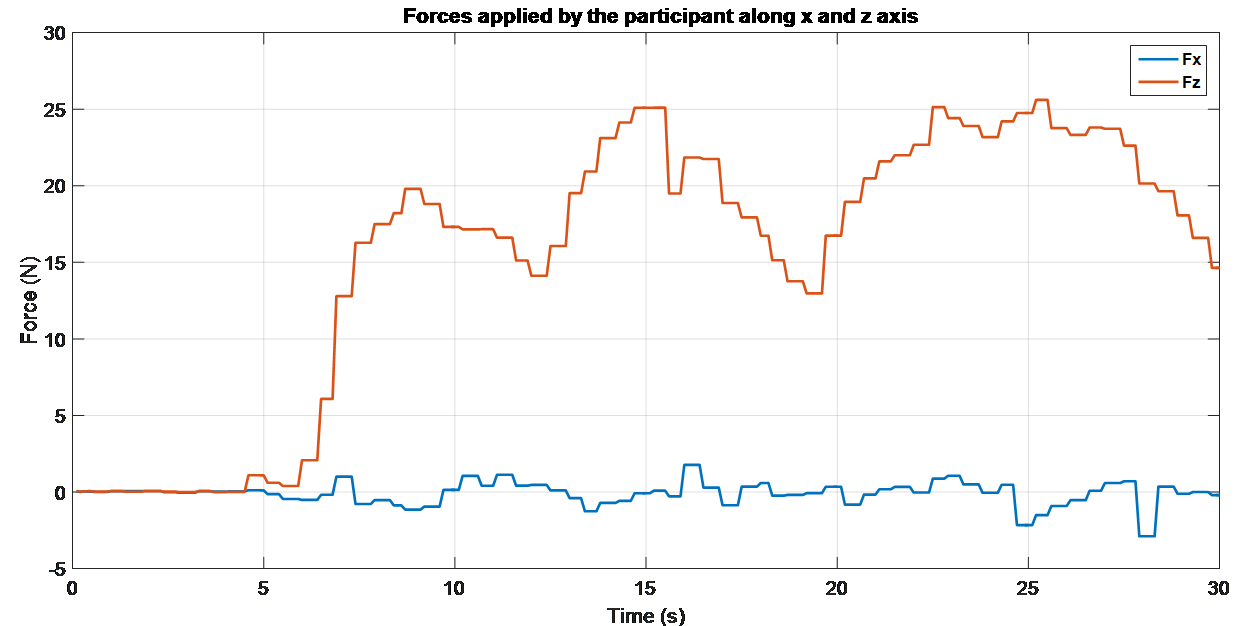
\includegraphics[width=.7\textwidth]{fext.png}
\caption{ External forces applied by the participant along the x and z axis are measured using the Haptic Master device.}
\label{externalforce}
\end{figure}

The observed torque behaviour in all the three joints of the planar model are presented in fig {\ref{torque}}. The initial joint torques are applied based on the input from the controller which later on combines with the output from the haptic master. The torque performance explains the movement followed in the planar model, with respect to the user applied forces. The torques profile stabilises at the end of 30seconds time window which is also in relation to the stabilised forces observed in fig. {\ref{externalforce}}.  
\begin{figure}[h!]
\centering
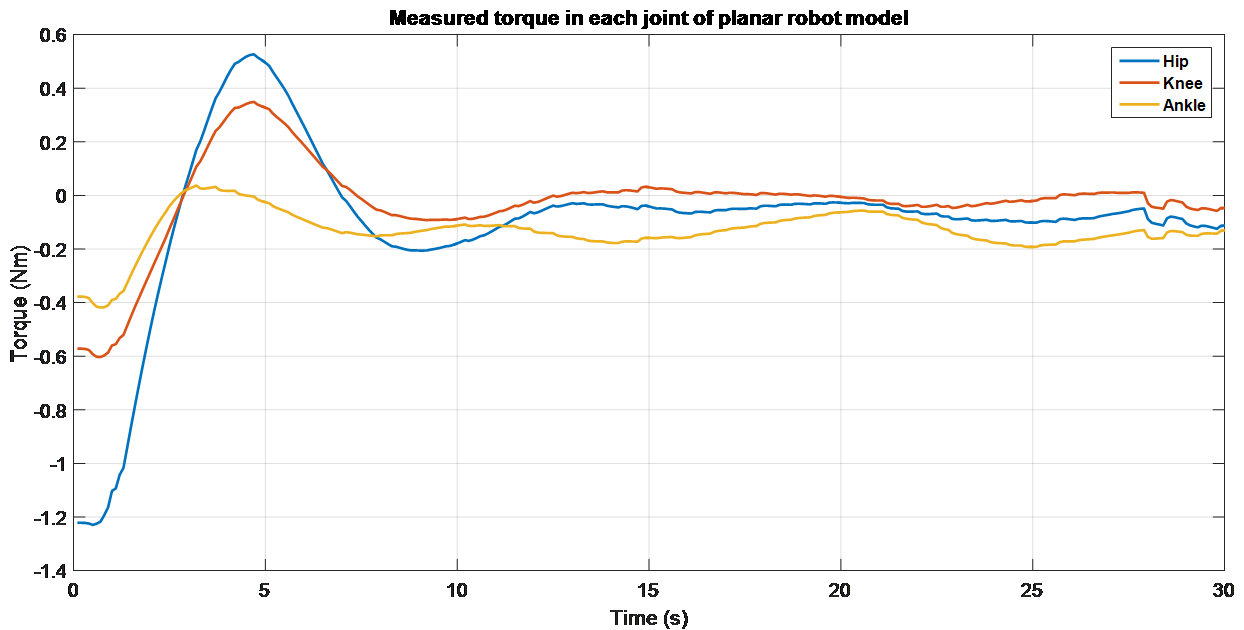
\includegraphics[width=.7\textwidth]{tau.png}
\caption{Resulting torque applied to the planar robot model, The torque performance varied depending on the External force applied by the user and the controller output.}
\label{torque}
\end{figure}

% Serena
\subparagraph*{Analysis of social and physical signals in human-robot interaction during assembly task}

We analyzed the social and physical signals exchanged by 56 human participants and the iCub during a collaborative assembly task. The experiments, performed by Serena Ivaldi at UPMC, were later analyzed during her time in TUD and INRIA.
First, we focused on social signals. In [Ivaldi et al., Int. Journal of Social Robotics 2016], we reported the analysis of results concerning the influence of individual factors in gaze and speech. We found that the more an individual is extrovert, the more he/she will tend to talk to the robot; the more an individual has a negative attitude towards robot, the less he/she will gaze at the robot’s face and the more he/she will tend to look at the robot’s hands, where the physical interaction occurs. In [Anzalone et al, Int. Journal of Social Robotics 2017] we also showed that it is possible to predict the extroversion of an individual from a thin slice of face to face interaction between the human and the robot, by taking into account several movement metrics.
We later started to analyze the physical signals, in particular the forces at the end-effectors of the robot (hands) where people were grasping the robot to drive and show the movement. We observed many interesting facts: the variance of median contact forces tis smaller in men than women; older people apply smaller forces; extroverts also apply small forces; by contrast, people with negative attitude towards interactions with robots (a subscale of NARS) apply bigger forces. We observed a visible difference between the demonstrations by the expert and the demonstrations provided by the participants, that were not robotics experts: the difference is highly visible, especially in terms of the variability of trajectories and different strategies adopted by the participants when moving the robot arms. Nevertheless, we observed a learning effect in the trajectories demonstrated by the participants: the smoothness of the movement, measured by the log-dimensionless jerk computed on the trajectories, increases across 3 trials in a significant way. A paper summarizing these results is currently in preparation.
